\documentclass{examen}
\usepackage{listings}
\begin{document}

\modulo{Lenguajes de marcas}


\pregunta{Dado el archivo XML de inventario, 
crear una hoja de estilo XSLT que transforme dicho archivo en el archivo XML que aparece a continuaci�n
}{3.5}
\begin{verbatim}
<inventario><!--Archivo de inventario-->
    <producto codigo="P1">
        <peso unidad="kg">10</peso>
        <nombre>Ordenador</nombre>
        <lugar edificio="B">
            <aula>10</aula>
        </lugar>
    </producto>
    <producto codigo="P2">
        <peso unidad='g'>500</peso>
        <nombre>Switch</nombre>
        <lugar edificio="A">
            <aula>6</aula>
        </lugar>
    </producto>
</inventario>
\end{verbatim}

\break
\begin{verbatim}
<!--Esto debe ser lo que devuelva el archivo XSLT para el inventario-->
<datos>
    <listacodigos>
        <codigo>P1</codigo>
        <codigo>P2</codigo>
    </listacodigos>
    <aulas>
        <aula>B-10</aula>
        <aula>A-6</aula>
    </aulas>
    <productos>
        <producto>
            Ordenador de 10kg
        </producto>
        <producto>
            Switch de peso 500g
        </producto>
    </productos>
</datos>

\end{verbatim}
\break
\pregunta{Dado el archivo XML cuyo nodo ra�z es {\tt listado} crear un archivo XSLT que lo convierta en una tabla HTML
como la mostrada en la figura. Obs�rvese que en dicha tabla solo deben aparecer los productos que pesen mas de 2100 kg y que a veces el peso
va en kilos y a veces en toneladas.}{6.5}
\begin{figure}[h]
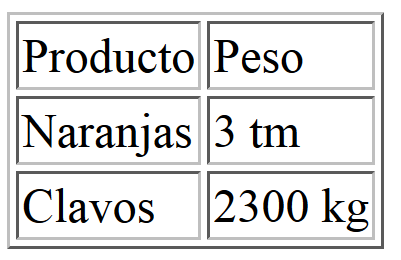
\includegraphics[scale=0.6]{examen-img/tabla_xslt.png}
\caption{Tabla resultado de transformar con XSLT}
\end{figure}
\begin{verbatim}
<listado>
    <perecederos>
        <fruta producto="Manzanas">
            <peso unidad='kg'>2000</peso>
            <caducidad>35 dias</caducidad>
        </fruta>
        <fruta producto="Naranjas">
            <peso unidad="tm">3</peso>
            <caducidad>22 dias</caducidad>
        </fruta>
    </perecederos>
    <noperecederos>
        <caja>
            <producto>Clavos</producto>
            <peso>
                <cantidad>2300</cantidad>
                <unidad>kg</unidad>
            </peso>
        </caja>
    </noperecederos>
</listado>
\end{verbatim}
\end{document}
